\chapter{DNSSEC}

En este capítulo se verá cómo funciona DNSSEC (Domain Name System Security Extensions) dentro del servidor, desde la generación de las claves criptográficas, pasando por distintos procecsos de firmas
para cada \texttt{RRSET}, hasta la creación e inserción de los registros \texttt{NSEC} y \texttt{DS}. 

Pero para poder comprobar que las respuestas DNS son auténticas y válidas, es necesario tener un cliente que pueda validar las respuestas DNSSEC, especificamente
usando la cadena de autentificación. En primera instancia, esta verificación se iba a realizar dentro del \texttt{stub-resolver} de la librería \texttt{dns-rust}, pero debido a que las funciones de parsing de la librería
están rotas (las funciones \texttt{to\_bytes} y \texttt{from\_bytes}), se decidió hacer todo de manera local. En un capítulo posterior se explicará por qué las funciones de parsing están rotas y 
cómo se podría solucionar.

\section{Servidor}

\subsection{Generación de llaves criptográficas}

El proceso de firma es complejo y requiere de dos pares de llaves criptográficas por cada zona: un par de llaves para firmar los datos (llaves ZSK : Zone Signing Key) y otro par de llaves para 
firmar las llaves ZSK (llaves KSK : Key Signing Key). Esto es requerido ya que DNSSEC utiliza un modelo de confianza basado en la jerarquía del DNS, donde cada zona firma sus registros
\texttt{DNSKEY} con su llave KSK, y la zona padre guarda un registro \texttt{DS} que apunta a la llave KSK de la zona hija, firmando este registro con su propia llave KSK. De esta manera, se 
puede construir una cadena de confianza desde la raíz del DNS hasta cualquier zona, verificando las firmas en cada nivel.

Para mayor claridad se muestra el siguiente diagrama que ilustra el proceso de firmas en DNSSEC:

\begin{figure}[H]
    \centering
    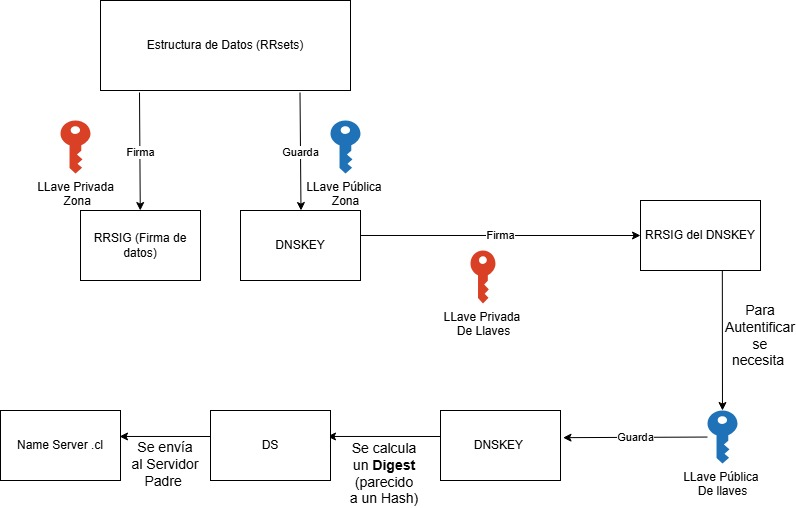
\includegraphics[width=1\textwidth]{diagramas/diagrama_encriptacion.jpg}
    \label{fig:dnssec-signing-process}
\end{figure}



El proceso de generación de las llaves criptográficas del sistema se realiza mediante el algoritmo RSA, utilizando la librería \texttt{rsa} del lenguaje Rust. Como 
este proceso debe hacerse una sola vez (y no cada vez que se ejecuta el servidor) se separó la lógica dentro de un archivo aparte llamado \texttt{generate\_keys.rs}, archivo
que se encuentra dentro del directorio \texttt{src/bin}, para que así pueda ser ejecutado de manera independiente.

El proceso de generación de las llaves criptográficas se realiza de la siguiente manera:
\begin{itemize}
    \item Se tiene una lista de zonas de los cuales se quieren generar las llaves criptográficas. En este caso, los dominios son \texttt{example.com},
          \texttt{niclabs.cl}, \texttt{.com}, \texttt{.cl} y \texttt{root} (raíz).
    \item Por cada dominio, se generan los dos pares de llaves criptográficas (KSK y ZSK) utilizando la función \texttt{generate\_keypair}
    \item Cada llave generada se guardan archivos dentro del directorio \texttt{keys/zona} a través de la función \texttt{write\_keys\_to\_disk}
\end{itemize}

\subsubsection{generate\_keypair}

En primer lugar, la función \texttt{generate\_keypair(bits)} recibe como parámetro el tamaño de la llave en bits (por ejemplo, 1024 o 2048). Dentro de la función, 
se instancia un generador de números aleatorios seguro del sistema operativo (\texttt{OsRng}), el cual provee la entropía necesaria para la generación de claves criptográficamente seguras, a 
partir de este generador se crea una llave privada RSA

Posteriormente, la llave pública se deriva directamente desde la llave privada usando el método \texttt{to\_public\_key()}.
El resultado de esta función es una tupla que contiene ambas llaves: \texttt{(RsaPrivateKey, RsaPublicKey)}.

\subsubsection{write\_keys\_to\_disk}

La función \texttt{write\_keys\_to\_disk(domain, zsk, ksk)} se encarga de almacenar físicamente las llaves generadas en disco.
Esta función recibe como parámetros el nombre de la zona (por ejemplo, \texttt{cl}) y los pares de llaves correspondientes al ZSK (Zone Signing Key) y KSK (Key Signing Key).

Dentro de la función, primero se crea un directorio con la estructura \texttt{keys/{domain}} para asegurar que exista la carpeta donde se guardarán los archivos PEM (Privacy Enhanced Mail), formato
comúnmente utilizado para almacenar llaves criptográficas. Posteriormente, se escriben las llaves en formato PKCS\#8 (estándar de representación de llaves en formato PEM) mediante los 
métodos \texttt{to\_pkcs8\_pem()} para las llaves privadas y \texttt{to\_public\_key\_pem()} para las llaves públicas.

Cada llave se almacena en un archivo independiente con nombres descriptivos:
\begin{itemize}
\item \texttt{zsk\_priv.pem}
\item \texttt{zsk\_pub.pem}
\item \texttt{ksk\_priv.pem}
\item \texttt{ksk\_pub.pem}
\end{itemize}

Aclarar que un nombre de carpeta NO puede ser "." (punto), por lo menos en Windows, ya que genera un error al intentar crear el directorio, esto obliga a renombrar la carpeta de la raíz a "root"

\subsection{Estructuras de datos para las llaves}

Una vez generadas las llaves y guardadas en formato PEM dentro de la carpeta \texttt{keys/zona} correspondiente, es necesario cargarlas en memoria
a través de alguna estructura global accesible desde cualquier parte del servidor. Para esto, se definieron las siguientes estructuras de datos

\subsubsection{ZoneKeyStore}

La estructura \texttt{ZoneKeyStore} es un mapa hash que asocia cada zona (representada como un string) con un puntero a su correspondiente conjunto de llaves criptográficas, que a su vez es otra
estructura llamada \texttt{ZoneKeys}. Esta estructura se define de la siguiente manera:

\begin{lstlisting}
    pub struct ZoneKeyStore {
        keys: HashMap<String, Arc<ZoneKeys>>,
    }
\end{lstlisting}

Se usa \texttt{Arc} (Atomic Reference Counting) para permitir que múltiples partes del programa puedan compartir acceso a las llaves de una zona sin necesidad de clonarlas.

La variable global accesible desde cualquier parte del servidor se define como:

\begin{lstlisting}
    pub static GLOBAL_ZONE_KEY_STORE: Lazy<ZoneKeyStore> = Lazy::new(|| {
        let mut store = ZoneKeyStore::new();

        let domains = ["example.com.", "niclabs.cl.", "com.", "cl.", "root."];

        for domain in &domains {
            let path = format!("keys/{}", domain);
            let zone_keys = ZoneKeys::load_from_path(&path);
            store.insert_zone_keys(domain.to_string(), Arc::new(zone_keys));
        }

        store
    });
\end{lstlisting}

La cual basicamente itera sobre la lista de zonas, carga las llaves desde el disco usando la función \texttt{ZoneKeys::load\_from\_path}
y las inserta en el ZoneKeyStore.

\subsubsection{ZoneKeys}

La estructura \texttt{ZoneKeys} almacena las cuatro llaves criptográficas necesarias para una zona DNSSEC: la llave privada y pública del ZSK (Zone Signing Key) 
y la llave privada y pública del KSK (Key Signing Key). Esta estructura se define de la siguiente manera:

\begin{lstlisting}
    pub struct ZoneKeys {
        zsk_priv: RsaPrivateKey,
        zsk_pub: RsaPublicKey,
        ksk_priv: RsaPrivateKey,
        ksk_pub: RsaPublicKey,
    }
\end{lstlisting}

Su metodo \texttt{load\_from\_path(path)} se encarga de leer los archivos PEM desde el disco, parsearlos con el método \texttt{from\_pkcs8\_pem} de la librería \texttt{rsa}
y crear una instancia de \texttt{ZoneKeys} con las llaves correspondientes.

\subsection{Inserción de DNSKEY's RRSETS en la estructura de datos}

Una vez que ya se tienen las llaves cargadas en memoria, se pueden utilizar para crear los registros \texttt{DNSKEY} necesarios para cada zona. Estos registros contienen las llaves públicas
utilizadas para verificar las firmas de los registros DNS, tanto del par ZSK como del par KSK.

Por lo que se debe insertar un \texttt{RRSET} de tipo \texttt{DNSKEY} por cada estructura de datos de cada zona. Esto se realiza en la función \texttt{insert\_dnskey\_rrsets}.

El algoritmo \texttt{insert\_dnskey\_rrset} crea un \texttt{RRset} para la zona con clase \texttt{IN}, tipo \texttt{DNSKEY} y el \texttt{TTL} dado por el proceso de parsing del masterfile. Luego
obtiene las claves desde la variable global \texttt{GLOBAL\_ZONE\_KEY\_STORE}, codifica las claves públicas con \texttt{encode\_rsa\_public\_key} y construye dos \texttt{DnskeyRdata}, los cuales 
tienen los siguientes campos:

\begin{itemize}
    \item \texttt{flags}: Indica el tipo de llave. El valor 256 indica una llave ZSK (Zone Signing Key) y el valor 257 indica una llave KSK (Key Signing Key). En este caso se usan ambos valores.
    \item \texttt{protocol}: Siempre es 3, según lo especificado en el RFC 4034.
    \item \texttt{algorithm}: Indica el algoritmo criptográfico utilizado. En este caso, se usa el valor 8, que corresponde a RSA/SHA-256.
    \item \texttt{public\_key}: Contiene la representación codificada de la llave pública en formato wire.
\end{itemize}

En cuanto al proceso de codificación de las llaves públicas RSA en el formato requerido por DNSSEC, se utiliza la función \texttt{encode\_rsa\_public\_key}, la cual
se encarga de codificar una clave pública RSA en el formato wire definido por el RFC 3110.

Primero obtiene los bytes del exponente (\texttt{e}) y del módulo (\texttt{n}) en orden big-endian. Luego, si el exponente tiene una longitud entre 1 y 255 octetos, 
este se representa con un solo byte; si supera los 255 bytes, se antepone un byte con valor 0 seguido de dos bytes que indican su longitud. 

Después de codificar la longitud, se concatenan los bytes del exponente y del módulo, formando la representación final que sigue la sintaxis del campo \texttt{public\_key} en los registros \texttt{DNSKEY}

Finalmente se insertan los datos a las estructuras correspondientes.

\subsection{Inserción de los RRSIG de los DNSKEY's RRSET}

Una vez insertados los registros \texttt{DNSKEY} en la estructura de datos, se procede a firmarlos utilizando la llave KSK (Key Signing Key), conforme a lo establecido en el RFC 4035, 
Sección 2.1.1. Esta firma es distinta de las que se aplican a los demás RRsets de la zona, los cuales se firman con la llave ZSK (Zone Signing Key).
La función \texttt{insert\_rrsig\_rrset\_dnskey} es la encargada de realizar este proceso.

En primer lugar, el algoritmo obtiene el conjunto de registros \texttt{DNSKEY} desde la estructura de datos y recupera la llave privada KSK almacenada en \texttt{GLOBAL\_ZONE\_KEY\_STORE}.
Luego, calcula el \texttt{key\_tag} de la KSK aplicando el algoritmo definido en el Apéndice B del RFC 4034, el cual consiste en sumar los bytes del \texttt{RDATA} del registro \texttt{DNSKEY} 
en formato wire y reducir el resultado a 16 bits. Este valor actúa como un identificador único de la clave utilizada en la firma.

Posteriormente, se construye la estructura \texttt{RRSIG\_Rdata}, completando los campos definidos en el RFC~4034, Sección~3.1. 
Cada uno de estos campos cumple una función específica dentro del registro de firma:

\begin{itemize}
    \item \textbf{\texttt{type\_covered}}: indica el tipo de registro DNS cubierto por la firma.  
    En este caso, su valor es \texttt{DNSKEY}, ya que la firma se aplica sobre el conjunto de claves públicas del dominio.

    \item \textbf{\texttt{algorithm}}: especifica el algoritmo criptográfico utilizado para generar la firma.  
    Se asigna el valor \texttt{8}, correspondiente a \texttt{RSASHA256}, conforme al RFC~4034.

    \item \textbf{\texttt{labels}}: representa la cantidad de etiquetas (labels) del nombre de dominio al que pertenece el RRSet.  
    Su valor se obtiene mediante la función auxiliar \texttt{count\_labels(zone\_name)}.

    \item \textbf{\texttt{original\_ttl}}: contiene el valor TTL original del \texttt{RRSet} firmado, copiado directamente desde el conjunto \texttt{DNSKEY}.

    \item \textbf{\texttt{signature\_inception}} y \textbf{\texttt{signature\_expiration}}: definen el intervalo de validez de la firma.  
    En esta implementación se establecen con valor \texttt{0}, ya que el servidor no implementa aún manejo de tiempo real ni soporte para zonas dinámicas.

    \item \textbf{\texttt{key\_tag}}: identifica de forma única la clave usada para la firma. En este caso se utiliza el valor calculado previamente a partir de la KSK.
    
    \item \textbf{\texttt{signer\_name}}: indica el nombre del propietario de la clave utilizada para la firma, correspondiente al dominio de la zona (\texttt{zone\_name}).
    
    \item \textbf{\texttt{signature}}: almacena la firma criptográfica generada sobre el \texttt{RRSet} de \texttt{DNSKEY}. A continuación se detalla el proceso para calcular este campo.
\end{itemize}

Para generar la \texttt{signature} se necesita firmar el \texttt{TBS} (To Be Signed), el cual sería la concatenación de los campos del \texttt{RRSIG} (exceptuando la misma \texttt{signature})
con el \texttt{DNSKEY} en versión canónica. Este proceso se realiza mediante la función auxiliar \texttt{build\_tbs\_data} siguiendo el orden establecido por el proceso de canonicalización de DNSSEC.

Finalmente, se utiliza la llave privada del par KSK para firmar el \texttt{TBS} utilizando el algoritmo RSA con SHA-256b y se añade el \texttt{RRSET} de \texttt{RRSIG} resultante a la estructura de datos del servidor.


\subsection{Creación e inserción de firmas y el manejo de casos bordes}

Después de insertar y firmar los registros \texttt{DNSKEY}, el siguiente paso consiste en firmar todos los demás \texttt{RRSET} presentes en la zona.
Naturalmente, los registros \texttt{RRSIG} no deben firmarse, ya que ellos mismos contienen las firmas de los conjuntos de registros.

Este procedimiento es prácticamente idéntico al proceso de firma de los \texttt{DNSKEY}, con la diferencia de que en este caso se utiliza la llave \texttt{ZSK} (Zone Signing Key) en lugar de la 
\texttt{KSK} (Key Signing Key), y se aplica a cada \texttt{RRSET} perteneciente a un dominio de la zona. Sin embargo, existen ciertos casos borde que deben manejarse cuidadosamente: 
los registros \texttt{NSEC}, los registros no autoritativos o de delegación, y los \texttt{wildcards}.

En primer lugar, el proceso de generación y firma de los registros \texttt{NSEC} es más extenso y se detalla en la siguiente sección.
En cuanto a los registros no autoritativos o de delegación (por ejemplo, los registros \texttt{NS} que apuntan a una zona hija), estos no deben ser firmados, ya que son responsabilidad de la zona delegada.
Para detectar estos casos dentro de la estructura de datos, se implementó la función \texttt{is\_authoritative\_rrset}, cuyo flujo general es el siguiente:

\begin{itemize}
    \item Verifica que el nombre del \texttt{RRset} pertenezca efectivamente a la zona. Si no está dentro de la zona, no se considera autoritativo.

    \item Evita firmar los \texttt{RRset} de delegación, es decir, los registros \texttt{NS} que no se encuentran en el apex de la zona.

    \item Evita firmar los \texttt{glue records}, es decir, registros \texttt{A} o \texttt{AAAA} asociados a una delegación, los cuales solo sirven para resolver los nombres de los servidores delegados.

    \item En cualquier otro caso, el \texttt{RRset} se considera autoritativo y debe ser firmado.
\end{itemize}

En el caso de los wildcards, su identificación es directa, ya que el nombre del \texttt{RRset} comienza con un asterisco (\texttt{*}).
Cuando esto ocurre, se debe restar uno al conteo de etiquetas (\texttt{labels}) del campo correspondiente en el \texttt{RRSIG}.
Esto permite que el resolver pueda reconocer que la respuesta proviene de un wildcard y validar correctamente su firma.
De no hacerlo, el cliente no podría distinguir el wildcard de un nombre explícito y la validación DNSSEC fallaría.

Esta regla está establecida explícitamente en el RFC 4035, Sección 5.3.2, que indica:

\begin{lstlisting}
"If the number of labels in an RRset's owner name is greater than the Labels field of the covering RRSIG RR,
then the RRset and its covering RRSIG RR were created as a result of wildcard expansion."
\end{lstlisting}

\subsection{Creación e inserción de los registros NSEC}

Los registros \texttt{NSEC} (Next Secure) son fundamentales en DNSSEC para proporcionar autenticación de ausencia de datos.
Estos contienen los siguientes campos:

\begin{itemize}
    \item \textbf{\texttt{next\_name}}: Indica el siguiente nombre de dominio en orden canónico dentro de la zona.
    \item \textbf{\texttt{type\_bitmap}}: Es un mapa de bits que señala los tipos de registros presentes para el nombre de dominio actual.
\end{itemize}

La función \texttt{create\_and\_insert\_nsec\_rrsets} construye e inserta todos los \texttt{NSEC RRSET} de la zona, siguiendo estrictamente lo especificado por los RFC 4034 y 4035. 
El proceso completo involucra dos tareas principales:

\subsubsection{Construcción de la lista de nombres para NSEC (NSEC owner names)}

El primer paso consiste en determinar exactamente cuáles nombres del archivo de zona deben poseer un \texttt{NSEC}. Esto se realiza mediante la función \texttt{gather\_nsec\_names}, 
la cual recorre toda la estructura interna de datos y selecciona únicamente aquellos nombres que corresponden a información autoritativa o a puntos de delegación. 
Esta filtración es esencial porque los registros \texttt{NSEC} describen únicamente nodos válidos dentro de la jerarquía DNS de la zona firmada. Una vez reunidos estos nombres, 
la lista se ordena en el orden canónico, siguiendo las reglas del RFC 4034 Appendix B.

\subsubsection{Construcción de los mapas de tipos}

Posteriormente, para cada nombre de esta lista se construye el campo \texttt{type\_bit\_maps}. 
Durante la iteración de los tipos presentes en un nombre, la implementación evita incluir todos los tipos considerados “pseudo‐tipos”, tales como \texttt{OPT}, \texttt{TSIG}, \texttt{ANY}, 
entre otros. Estos tipos no forman parte de la información firmada ni pueden aparecer legítimamente en un bitmap de un NSEC, tal como lo establece el RFC 4034 4.1.2. 
Luego, dependiendo del tipo de nodo, existen reglas especiales. Si el nombre es un punto de delegación (es decir, contiene un \texttt{RRset} \texttt{NS} pero no es el apex), solo se deben incluir en el 
bitmap los tipos \texttt{NS} y \texttt{DS}. Esto se debe a que, según el RFC 4035 2.3, el servidor padre no es autoritativo para el resto de los registros del dominio delegado y, 
por lo tanto, no debe afirmar su existencia mediante un NSEC. En contraste, si el nombre corresponde a información completamente autoritativa, se incluyen todos los tipos válidos 
presentes en el nodo. En ambos casos, de manera obligatoria, se agrega también el tipo \texttt{NSEC} al bitmap, ya que cada nombre que tiene un NSEC necesariamente debe anunciarlo explícitamente, 
como lo dicta el RFC 4034 4.1.2.


Finalmente, con el nombre actual, el siguiente nombre en orden canónico y el bitmap resultante, se construye la \texttt{RData} \texttt{NSEC}. El \texttt{TTL} del registro se 
toma desde el campo “minimum TTL” del \texttt{SOA} del apex, siguiendo la recomendación del RFC 4034 2.3.4. Con toda esta información se produce un nuevo \texttt{RRset} de tipo \texttt{NSEC}, 
el cual se inserta en la estructura de datos de la zona.

\subsection{Inserción de RRSIGS para los NSEC RRSET}

El proceso de construcción de los registros \texttt{NSEC} es, en esencia, el mismo que el descrito previamente en la subsección \texttt{Creación e inserción de firmas y el manejo de casos bordes}. 
Sin embargo, surge una pregunta natural: ¿por qué las firmas \texttt{RRSIG} correspondientes a los \texttt{NSEC} se generan en un paso separado, en lugar de ser firmadas junto con el resto de 
los \texttt{RRSET}? La razón es estructural. Los registros \texttt{NSEC} deben reflejar con precisión todos los tipos existentes en cada nombre, y eso incluye los \texttt{RRSIG}. 
En otras palabras, el mapa de tipos (\texttt{type\_bit\_maps}) de un \texttt{NSEC} debe considerar la presencia de las firmas ya generadas. Por este motivo, los \texttt{RRSIG} de los demás 
\texttt{RRSET} deben existir antes de crear los \texttt{NSEC}. Si se intentara firmar todo en un solo paso, los \texttt{NSEC} no podrían incluir los tipos correctos, produciendo un conjunto 
inconsistente e inválido bajo DNSSEC. Debido a esta dependencia lógica, la firma de los \texttt{NSEC} se ejecuta necesariamente como una fase posterior y separada.

\subsection{Creación del RRSET DS para la zona padre}

Un registro \texttt{DS} (Delegation Signer) es un tipo especial de registro DNS que se utiliza en DNSSEC para establecer una cadena de confianza entre una zona padre y una zona hija.
El cual contiene los siguientes campos:

\begin{itemize}
    \item \textbf{\texttt{key\_tag}}: Identificador único de la clave pública de la zona hija.
    \item \textbf{\texttt{algorithm}}: Algoritmo criptográfico utilizado por la clave pública.
    \item \textbf{\texttt{digest\_type}}: Tipo de función hash utilizada para generar el digest.
    \item \textbf{\texttt{digest}}: Resultado de aplicar la función hash a la concatenación del nombre canonico de la zona hija y su llave pública.
\end{itemize}

La construcción del RRSET \texttt{DS} se realiza en la función \texttt{build\_ds\_rrset}. Para ello
primero obtiene el \texttt{DNSKEY RRSET} del apex de la zona y prepara un nuevo \texttt{RRSET} \texttt{DS} con el mismo nombre, clase y TTL. Luego, recorre cada registro \texttt{DNSKEY} y 
selecciona únicamente aquellos que corresponden a la clave KSK. Para cada llave calcula el \texttt{key tag} y genera el valor del 
\texttt{digest} siguiendo las especificaciones del RFC 4509, concatenando el nombre de dominio en forma canónica con el RDATA del \texttt{DNSKEY} y aplicando la función hash dada según el \texttt{digest\_type}. 
Con esta información se construye la estructura \texttt{DsRdata}, que posteriormente se inserta como registro dentro del \texttt{DS RRSET}. Finalmente, el \texttt{RRSET} resultante se 
retorna para que pueda ser insertado en la estructura de datos de la zona padre.

El servidor no tiene acceso directo a la zona padre, por lo que al generar el \texttt{RRSET DS}, este se imprime en consola, se copian los datos y se insertan manualmente en el 
master-file de la zona superior. Esto coincide con la práctica actual de los servidores DNSSEC, ya que no existe todavía un mecanismo estandarizado y ampliamente adoptado para que los registros DS 
se envíen automáticamente al progenitor.

En la reunión ICANN 84 (Dublín, 25-30 de octubre de 2025) se abordó precisamente este tema en el contexto del taller  “Towards an Industry Best Practice for DS Automation” presentado por Peter 
Thomassen (deSEC), donde se revisaron estadísticas de adopción y los desafíos operativos para la automatización del envío de DS.

\section{Resolver}

Es fundamental verificar que las firmas generadas por el servidor sean correctas dentro del contexto de \texttt{DNSSEC}. Para ello, se implementó completamente la lógica de validación de firmas y 
de la cadena de autenticación. Originalmente, este proceso iba a realizarse dentro del \texttt{stub-resolver} de la librería \texttt{dns-rust}; sin embargo, debido a problemas en sus funciones 
internas de parsing, se optó por efectuar toda la validación localmente, replicando con precisión el flujo que tendría un \texttt{stub-resolver} real.

El proceso de autenticación debe distinguir entre varios escenarios posibles en una respuesta DNSSEC:

\begin{itemize}
\item Respuestas con datos en la sección \texttt{Answer} y sus \texttt{RRSIG} asociados.
\item Respuestas con código \texttt{NXDOMAIN}.
\item Respuestas \texttt{NO\_DATA}.
\item Respuestas originadas por consultas \texttt{DNSKEY}.
\item Respuestas generadas a partir de \textit{wildcard expansion}.
\end{itemize}

Para gestionar correctamente cada caso, se definió la función \texttt{dnssec\_authentification}, la cual recibe la consulta DNS original y retorna true si la respuesta es válida bajo DNSSEC, 
o false en caso contrario. El flujo general de esta función es el siguiente:

\begin{itemize}
\item En primer lugar, se ejecuta la función \texttt{lookup\_data} con \texttt{DNSSEC} habilitado, obteniéndose así la respuesta completa que será 
      inspeccionada para determinar qué mecanismo de validación corresponde aplicar.

\item Si el código de respuesta en el \texttt{Header} es \texttt{NXDOMAIN}, significa que el nombre consultado no existe en la zona.  
      En este caso se activa el proceso de autenticación basado en pruebas \texttt{NSEC} de inexistencia de dominio, mediante \texttt{nxdomain\_authentication\_process}.

\item Si el código es \texttt{NOERROR}, pero la sección \texttt{Answer} está vacía y la sección \texttt{Authority} contiene un registro \texttt{NSEC}, la respuesta corresponde al caso \textit{NO\_DATA}.  
      Para validar esta situación, se ejecuta \texttt{nodata\_authentication\_process}, el cual verifica la ausencia del tipo consultado mediante la prueba NSEC apropiada.

\item Si la consulta original corresponde al tipo \texttt{DNSKEY}, se activa el modo especial de autenticación que utiliza la KSK.  
      En este caso se invoca \texttt{authentification\_process} con la bandera \texttt{dnskey\_mod} en \texttt{true}.

\item Si no se cumplen las condiciones anteriores, se analiza la presencia de registros \texttt{RRSIG} en las secciones \texttt{Answer} y \texttt{Authority}.  
      Luego, se compara la cantidad de labels del nombre de dominio del RRset con el campo \texttt{labels} contenido en la firma \texttt{RRSIG}.  
      Si el número de labels del dominio es mayor que el valor en el \texttt{RRSIG}, se trata de una respuesta producida por \textit{wildcard expansion}.  
      En este caso, se ejecuta \texttt{wildcard\_authentication\_process}.

\item Si no se detecta wildcard, pero al menos un \texttt{RRSIG} existe, la respuesta corresponde a un caso de validación estándar, por lo que se invoca \texttt{authentification\_process}.

\item Finalmente, si la respuesta no contiene ningún \texttt{RRSIG}, no existe información criptográfica que validar.  
      El proceso falla explícitamente retornando \texttt{false}, pues la respuesta no cumple los requisitos de seguridad DNSSEC.
\end{itemize}

El siguiente diagrama de flujo ilustra visualmente este proceso:

\begin{figure}[H]
    \centering
    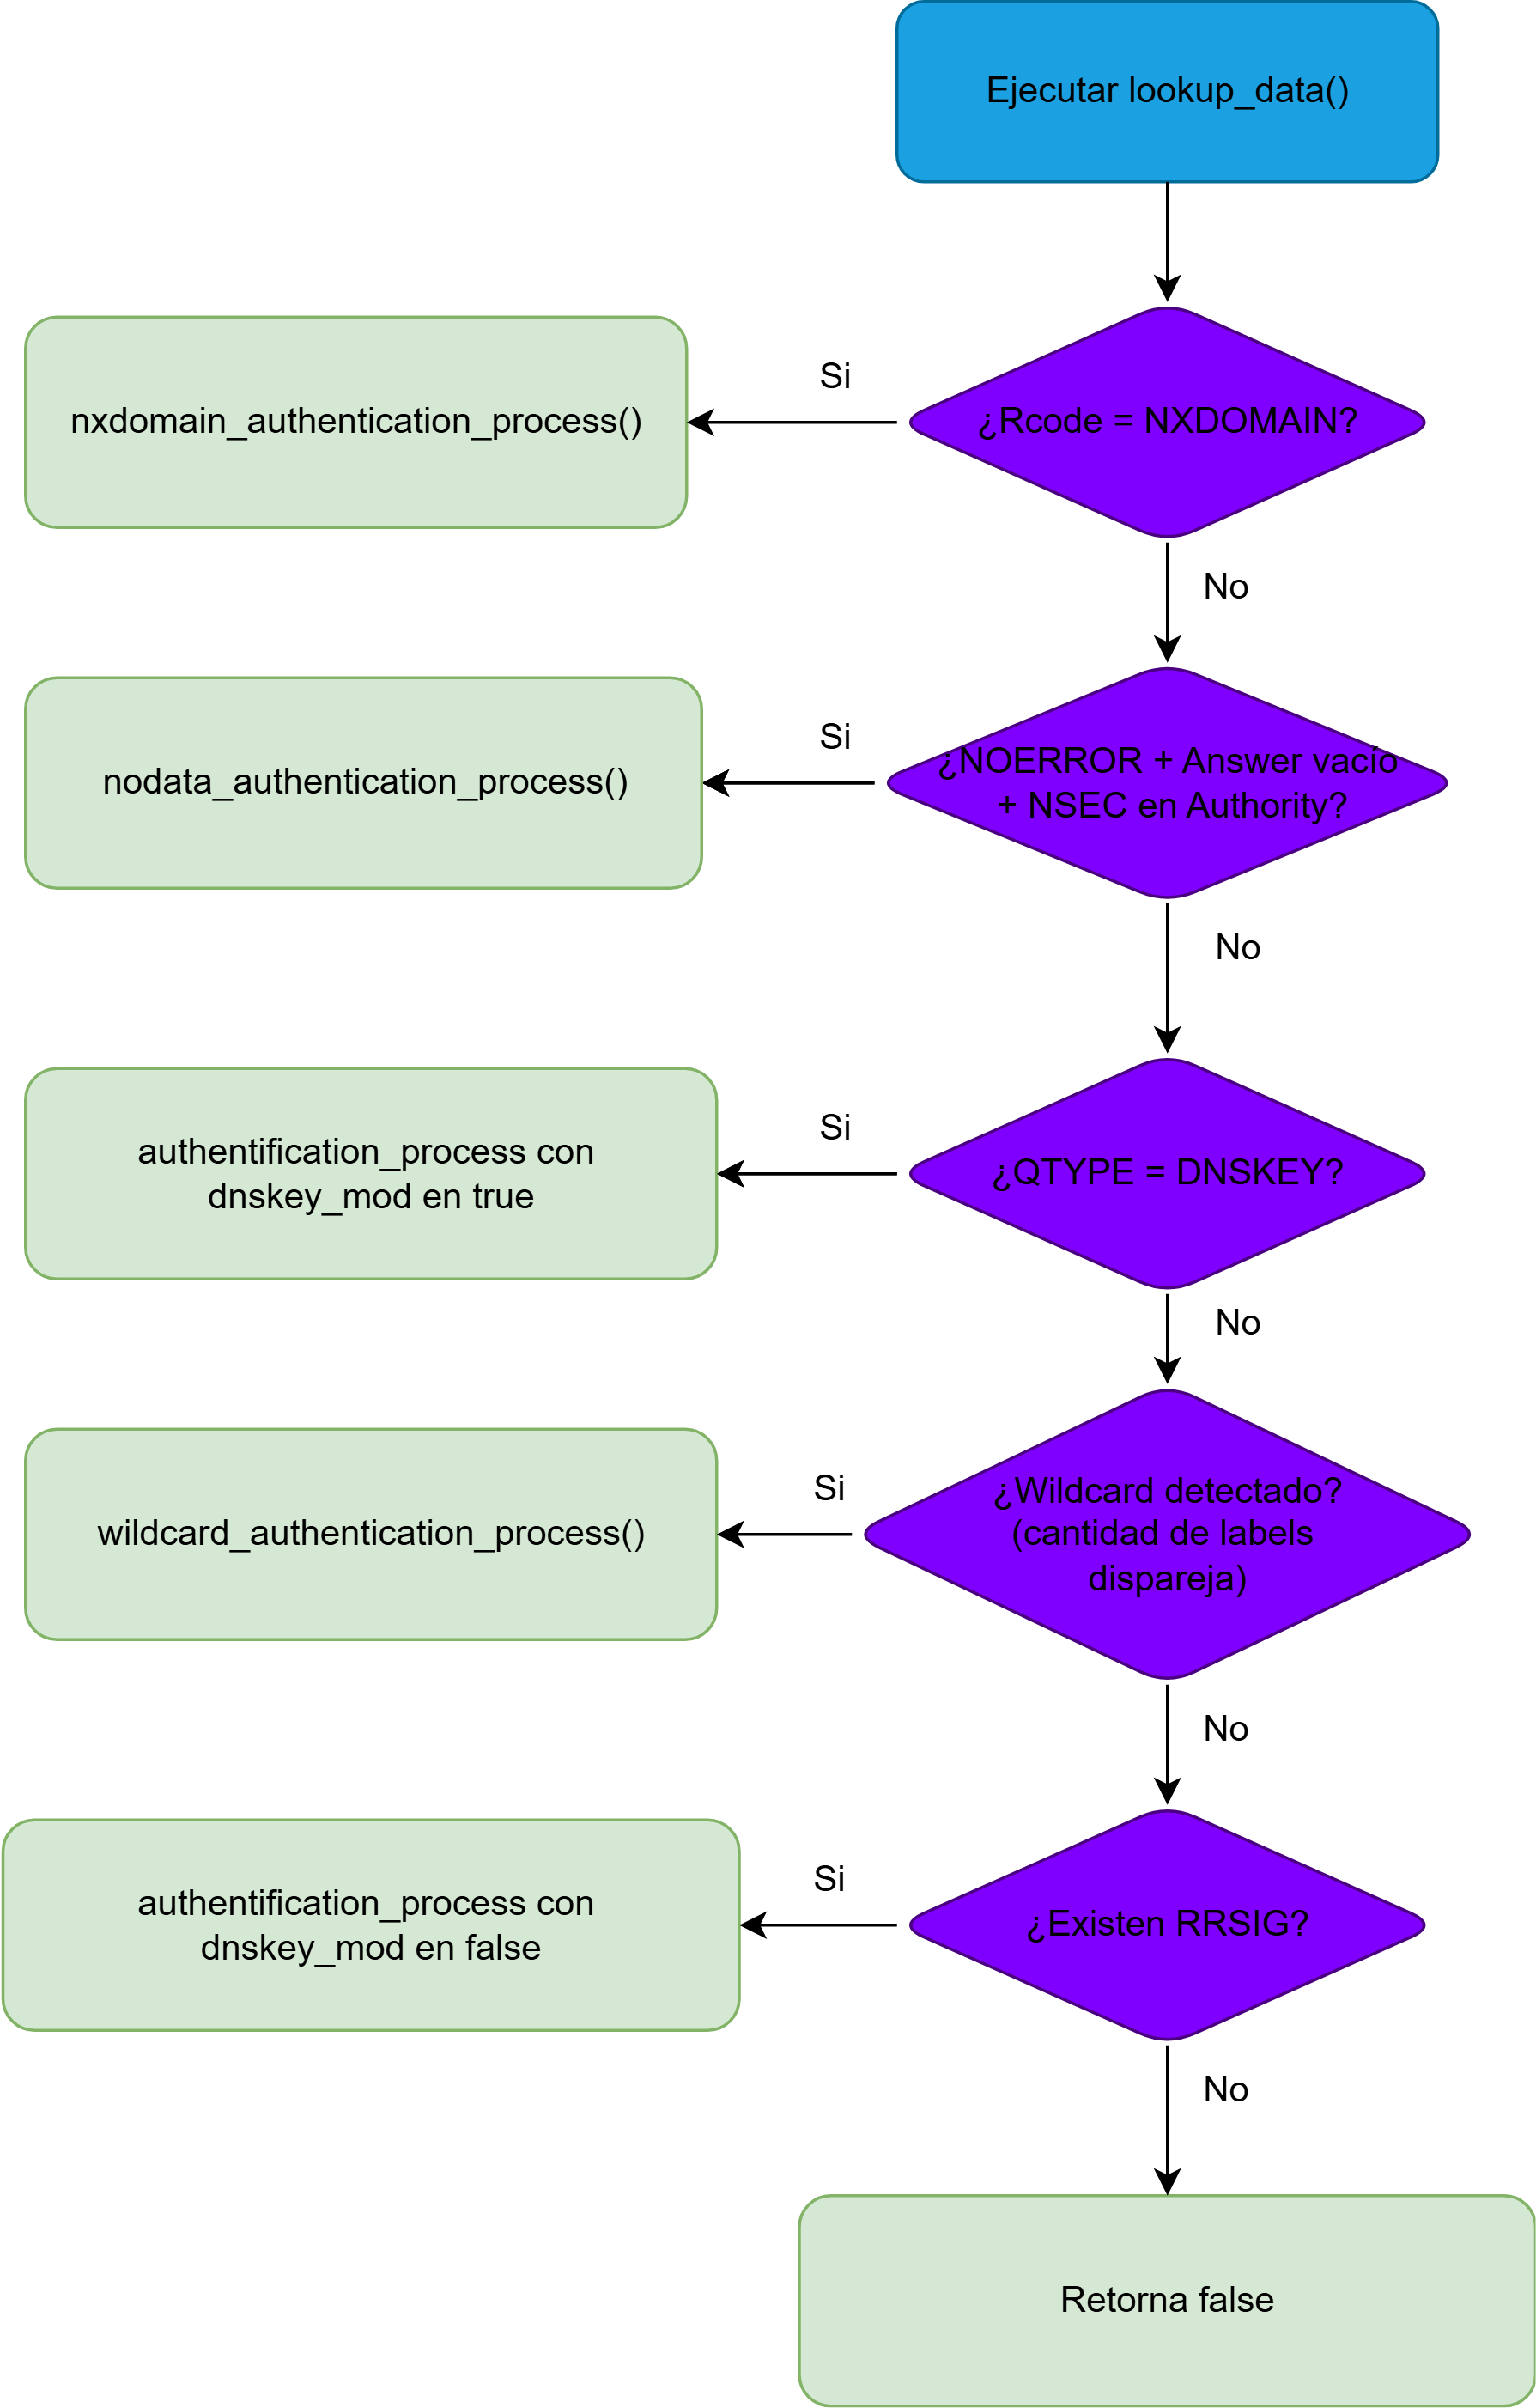
\includegraphics[width=0.6\textwidth]{diagramas/dnssec_auth.png}
    \label{fig:dnssec-resolver-flow}
\end{figure}

